Als Amazon, anfangs noch \emph{cadabra.com}, am 5. Juli 1994 von Jeff Bezos und seiner Frau McKenzie gegründet wurde, hatte wahrscheinlich niemand die Vision eines marktführendem Online-Unternehmens im Kopf - im Gegensatz, Amazon war ursprünglich ein Online-Buchhandel für bestimmte, seltene Bücher\cite[S. 17]{Graf}. Trotz der kleinen Zielgruppe wuchs das Unternehmen in den folgenden Jahren bedeutend: schon zwei Jahre später wurden Aktien angeboten, außerdem wurde anfangs noch fast der komplette Gewinn reinvestiert\cite{Rosoff}, was das Aufkaufen ganzer Unternehmen schon 4 Jahre nach der Gründung ermöglichte, bespielsweise von \emph{pets.com} und \emph{overstock.com}\cite{ChannelAdvisor}. Mit der Zeit expandierte die Firma in viele weitere Gebiete: Cloud Computing mit \ac{AWS} 2002 sowie Musik mit einem Online-Musik-Store und Lebensmittel mit AmazonFresh im Jahr 2007\cite{Sherman, ChannelAdvisor}. Auch bezüglich des Onlinehandels breitete Amazon ab 2000 nach und nach die Produktauswahl aus, wodurch sich der darmalige Buchhandel zu dem heutigen Onlineversandhandel für fast alle Produktereiche entwickelte. Ein wichtiger Schritt zu diesem Ziel war das Ermöglichen von Drittanbieter-Verkäufen ab dem 30. September 1999, was die Bekanntheit und Anzahl der Verkäufe erheblich steigerte\cite{Sherman}. Zudem ermöglich es der Firma, ein breiteres Produktsegment anzubieten sowie Provisionen zu erhalten, während Probleme wie Kapitalbildung und Lagerplätze an dritte Händler ausgelagert werden\cite[S. 50]{evilcom}. Außerdem wurden weitere Technologien wie Amazon Prime und AmazonBasics entwickelt, die den Onlinehandel und -versand unterstützen\cite{ChannelAdvisor}, aber auch alleinstehende Projekte, wie Kindles, das Fire Phone oder Smart-Home-Geräte\cite{Sherman}.
Die derzeitige Strategie bezüglich des Oninehandels beschrieb Bezos, als "Virtuos Cycle" betitelt, schon 2001  mit folgender Zeichnung\cite{zentail}:

%IST NICHT IMMER DA WO ES SOLL WENN ES ZB NICHT AUF DIE SEITE PASST

\begin{figure}[h]
    \begin{center}
        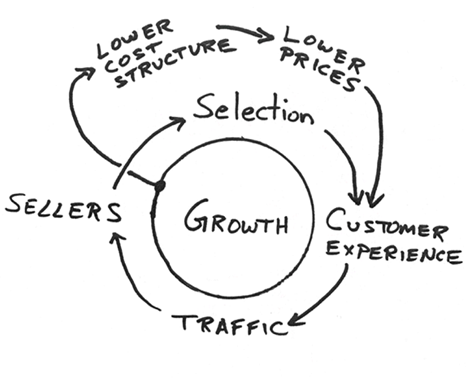
\includegraphics[width=8cm]{media/Fabian-vicious-cycle.png}
        \caption{Amazon's Vicious Cycle}
        \label{vicious-cycle}
        \bildquelle Jeff Bezos, September 2001 %Learn from the Bezos Virtuous Cycle: Leverage and Invest in Infrastructure, www.zentail.com, abgerufen August 2020% https://tinyurl.com/yyu2zz29 DATUM???
    \end{center}
\end{figure} 

Dabei schafft breit gefächerte Produktsegment(Selection) eine positive Kundenerfahrung(Customer Experience), die weitere Verkäufe und Verbreitung durch z. B. Empfehlungen(Traffic) hervorruft. Durch diese hohe Kundenanzahl ist die Plattform wiederrum attraktiver für Drittanbieter und Herstellern(Sellers), die weitere Produkte anbieten und das Produktsegment erweitern. Dieser Teil ist an sich nicht wirklich außergewöhnlich, da viele andere Onlineanbieter eine ähnliche Strategie verfolgen. Jedoch hebt sich Amazon damit ab, ungewöhnlich hohe Summen zu investieren, um Kosten(Lower cost structure) und somit auch Produktpreise(Lower prices) zu senken\cite[S. 26f]{Graf}. Amazon schaffte so auch ein neues Konsumverhalten, das "Amazon Commerce" - Graf und Schneider beschreiben es in ihrem Buch als ein

\begin{quote}
    "[...] komplett neues Kaufverhalten, das sich nicht mehr an Anbietern oder konkreten Produkten orientiert, sondern allein am Zweck [...], den das gewünschte Produkt erfüllen soll."\cite[S. 42]{Graf}
\end{quote}

Die genannten Punkte ermöglichten es Amazon, sich als weltweit bekannten und benutzten Onlineversandhandel zu etablieren - jedoch haben sie auch einige Probleme hervorgerufen. Beispielsweise führte die konstante Niedrigpreispolitik\cite[Abb. 5]{Desjardins} zum Einsparen von Ausgaben in fast allen Gebieten - auch im Bezug auf Angestellte\cite[S. 6]{Apicella}. So werden insbesondere in der Weihnachtszeit Leiharbeiter eingestellt. In der ARD-Reportage "Ausgeliefert! Leiharbeiter bei Amazon" wird 2013 gezeigt, wie deren Arbeitsalltag aussah: Zu siebt wird in einer Ferienwohnung übernachtet, oft bekommen die Angestellten nur wenige Stunden Schlaf. Jeden Tag aufs neue ist es unsicher, ob man gebraucht wird - wenn nicht, gibt es keinen Lohn. Mitarbeiter der Dienstleistungsgewerkschaft Ver.di und Amazons erklären, dass 2013 in Koblenz circa 3100 von 3300 Arbeitern befristet angestellt waren\cite{Ausgeliefert}.
Außerdem existiert ein hoher Grad an Überwachung und Kontrollen, wie Apicella in ihrer Studie andhand der Stadt Leipzig beschreibt:

\begin{quote}
    "Die Verkaufsarbeit durchläuft dabei einen Prozess der [...] vollständige[n] Überwachung und Disziplinierung der Beschäftigten[...].\cite[S. 29]{Apicella}"
\end{quote}

Dementsprechend sind Streiks bei Amazon keine Seltenheit: Beispielsweise streikten Angestellte in Deutschland zwei Monate nach der besagten Reportage unter dem Motto "Wir sind keine Roboter" gegen niedrige Löhne, befristete und allgemein schlechte Arbeitsverhältnisse sowie die starke Digitalisierung der Arbeit\cite[S. 6]{Apicella}. Amazon reagierte in den folgenden Jahren mit mehreren Lohnerhöhungen, jedoch exestieren noch vereinzelt Streiks, da die Arbeitsbedingungen anscheinend immer noch problematisch sind\cite{JGraf}. So schrieb Amazon z. B. 175000 neue Stellen in Folge der Corona-Krise und einem 32\%-igem Verkaufszuwachs aus - nicht nur, weil mehr Arbeiter als vorher gebraucht werden, sondern auch weil einige Angestellte aufgrund von "unsicheren Bedingungen" sich weigerten, zu ihrem Arbeitsplatz zu erscheinen\cite{Theweek}.

Innerhalb der letzen 26 Jahre hat Amazon sich von einem Online-Buchhandel zu einem weltweiten Onlinehändler fast alle Produktklassen entwickelt. Außerdem bietet die Firma heute auch andere Dienste an, wie z. B. Cloud Computing mit \ac{AWS}. Jedoch steht das Unternehmen bezüglich der Arbeitsbedingungen seit fast einem Jahrzehnt in der Kritik.
